  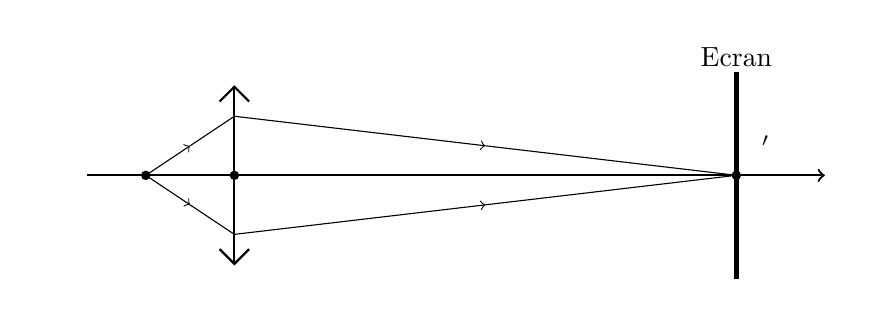
\begin{tikzpicture}[scale=0.75]
    \clip (-2,-2) rectangle (12,2.5) ; %Les dimensions de l'image
    \draw [->,thick] (-1,0) -- (11.5,0) ; %% L'axe optique
    \draw [thick] (1.5,-1.5) -- (1.5,1.5)  ; %% Le corps de la lentille 
    
    \draw [thick] (1.25,-1.25) -- (1.5,-1.5) -- (1.75,-1.25)
                         (1.25,1.25) -- (1.5,1.5) -- (1.75,1.25) ;                    %Lentille 
                         
  \filldraw [black] (0,0) circle (2pt) node at (0,0.5) {$\ptA$} ; %L'objet
    \filldraw [black] (1.5,0) circle (2pt) node[above right] {$\ptO$} ; %Le centre optique
  \filldraw [black] (10,0) circle (2pt) node at (10.5,0.5) {$\ptA'$} ; %L'image
      
  \draw [ultra thick] (10,-1.75) -- (10,1.75)  ; %% L'écran
  
  \draw [->,thin] (0,0) -- (0.75,0.5)  ; %Rayon 1
  \draw [thin] (0.75,0.5) -- (1.5,1)  ; %Rayon 1
  \draw [->,thin] (0,0) -- (0.75,-0.5)  ; %Rayon 2
  \draw [thin] (0.75,-0.5) -- (1.5,-1)  ; %Rayon 2
  \draw [->,thin] (1.5,1)  -- (5.75,0.5)  ; %Rayon 3
   \draw [thin] (5.75,0.5)  -- (10,0)  ; %Rayon 3
  \draw [->,thin] (1.5,-1)  -- (5.75,-0.5)  ; %Rayon 4
   \draw [thin] (5.75,-0.5)  -- (10,0)  ; %Rayon 4
   
  \node at (10,2) {Ecran}  ; %Légende1
  
      
  \end{tikzpicture}